\documentclass[conference]{IEEEtran}
\renewcommand\IEEEkeywordsname{keywords}
\usepackage{graphicx}
\usepackage{epstopdf}
\usepackage{float}
\usepackage{amssymb}
\usepackage{multirow}
\usepackage[english]{babel}
\usepackage{algorithmic,algorithm}
\renewcommand{\algorithmicrequire}{\textbf{Input:}}
\renewcommand{\algorithmicensure}{\textbf{Output:}}
\usepackage{enumerate}
\usepackage{lipsum}% http://ctan.org/pkg/lipsum
\hyphenation{op-tical net-works semi-conduc-tor}
\usepackage{booktabs}
\usepackage{amsmath}
\usepackage[smallscripts]{moresize}
%\usepackage[numbers,sort&compress]{natbib}
\usepackage[numbers,sort]{natbib}
\usepackage[most]{tcolorbox}
%\usepackage{ctable}

\begin{document}

\title{Enhancing Crop Health with Image-based Disease Detection in Bell Pepper Plants}
%%%%%%%%%%%%%%%%%%%%%%%%%%%%%%%%%%%%%%%
% \author{\IEEEauthorblockN{Utpal Kant Singh, Rajnish Kumar, Saurabh Kumar, Shibasish Kar, Santos Kumar Baliarsingh}

% \IEEEauthorblockA{School of Computer Engineering,
% KIIT Deemed to be University, Bhubaneswar, 751024, India}
% \{20051117, 2005118, 20051096, 2005335, santos.baliarsinghfcs\}@kiit.ac.in
% }
%%%%%%%%%%%%%%%%%%%%%%%%%%%%%%%%%%%%
\author{\IEEEauthorblockN{Utpal Kant Singh}
\IEEEauthorblockA{School of Computer Engineering\\
KIIT Deemed to be University,\\ Bhubaneswar, India 751024\\
Email: utpalkant.4855@gmail.com}
\and
\IEEEauthorblockN{Vishal R. Satpute}
\IEEEauthorblockA{Department of Electronics and \\Communication Engineering\\
VNIT, Nagpur, India 440010\\
Email: vrsatpute@ece.vnit.ac.in}
}
%%%%%%%%%%%%%%%%%%%%%%%%%%%%%%%%%%%%%%%%%%%%%


\maketitle

\begin{abstract}

India has a large-scale bell pepper industry that benefits from the tropical environment of the nation. However, a number of factors, such as climatic conditions, might have a negative impact on their growth and output. The production of bell pepper crops is seriously threatened by plant diseases, which can also result in large financial losses. Bell pepper plant disease detection using conventional techniques has been shown to be ineffective and time-consuming. Effective illness management depends on early identification. In order to effectively diagnose illnesses in bell pepper plants, this study explores the possibilities of deep learning techniques, especially convolutional neural networks (CNNs), in conjunction with computer vision technology. The outcomes show the viability of the suggested method, with an amazing average illness classification accuracy of 98\%. \\

 
\end{abstract}


\begin{IEEEkeywords}
Deep Learning, Machine Learning, Potato Leaf Disease Detection, Convolutional Neural Network, 
\end{IEEEkeywords}
 
\IEEEpeerreviewmaketitle



\section{Introduction}



\subsection{Motivation}
As farmers grow a variety of crops to suit the nation's agricultural demands, bell pepper farming is crucial to the Indian economy. The vulnerability of bell pepper plants to diseases, however, can cause substantial reductions in crop output and quality. To protect their livelihoods, farmers must identify these illnesses early and begin treatment. Commonly used in conventional disease management strategies are pesticides, which have a negative impact on the environment. Therefore, by lowering dependency on chemical treatments, early disease identification encourages sustainable agriculture practises. Additionally, several bell pepper infections can endanger human health as a result of tainted food or exposure to pollutants. certain hazards can be reduced with prompt diagnosis and treatment of certain illnesses. It is crucial to use precise and trustworthy automated methods to detect illnesses in bell pepper plant leaves since manual inspection-based methods are expensive and resource-intensive. \\ 

The fields of object identification and picture classification have seen a substantial revolution since the introduction of CNNs. It is possible that the use of CNNs in disease detection may completely change how we recognise and treat plant illnesses, particularly those that harm bell pepper plants. Due to early identification made feasible by CNNs, crop losses may be efficiently reduced and total production can be raised. CNNs minimise mistakes that might happen during visual examinations by offering correct diagnoses, which also lessens reliance on human specialists. Additionally, the use of CNNs in automated illness identification has the potential to greatly reduce costs and turnaround times, especially in areas with limited resources. This readily available and reasonably priced technology can assist farmers in overcoming obstacles brought on by knowledge and resource limitations, resulting in enhanced bell pepper plant cultivation results.\\ 

By using CNNs for automated illness detection, it is possible to significantly reduce the costs and turnaround times involved with traditional diagnostic methods. This is especially important in underdeveloped countries where there are little resources and experts available for properly identifying and treating plant diseases. CNNs provide a more accessible and affordable method of diagnosis, improving accessibility and affordability for farmers.

\subsection{Contributions}
\begin{itemize}
    \item A convolutional neural network (CNN) architecture based on deep learning is used to construct a system for categorising diseases affecting potato leaves. The system's primary objective is to precisely and properly categorise the many illnesses that affect potato plants.
    \item In testing and comparisons, the CNN model, which is recommended for the classification of potato plant leaf diseases, surpasses more complex models, illuminating its extraordinary effectiveness.
    \item The effectiveness and usability of the suggested CNN-based approach are evaluated by experiments on a publically available dataset of potato plant leaf diseases. The experimental results offer crucial information on the potential applications of the proposed method for disease diagnosis and classification in agriculture.\\
\end{itemize}
 
This work aims to assess the potential of CNNs for automatically detecting illness in bell pepper leaves. Farmers and the entire world's food supply chain would gain if the results of this study were used to the development of more precise and effective techniques of spotting diseases in bell pepper crops.


\section{Related Works}
Despite being a well-liked and nutritious crop, bell peppers are prone to a variety of ailments that, if not adequately identified and treated, can cause considerable crop output losses. In order to solve this problem, scientists have started automating the identification and classification of diseases in bell pepper plants using deep learning methods, particularly CNNs.\\

The early detection and efficient management of potato leaf diseases are critical for minimizing their impact. Asif et al. \cite{9316021} propose a model that utilizes image processing techniques to accurately identify and detect diseases in potato leaves. Among various machine learning algorithms, the Convolutional Neural Network (CNN) model is selected for its exceptional performance in image classification tasks. The study incorporates five different algorithms, including AlexNet, VggNet, ResNet, LeNet, and a Sequential model developed by the authors. The model is trained using both healthy and diseased leaf images to differentiate between normal and abnormal aspects of potato leaves. Through the implemented algorithm, the model achieves an impressive precision of 97\% in classifying potato plant leaves as either diseased or healthy. This research emphasizes the importance of disease detection in potato plants and highlights the effectiveness of the proposed CNN-based model in accurately identifying potato leaf diseases.\\


In order to achieve sustainable agricultural development, it is essential to conduct research in the field of plant disease diagnosis, leveraging advancements in agricultural technology and artificial intelligence. Diseases such as early blight and late blight have a significant impact on potato crops, and the manual identification of these leaf diseases can be a time-consuming and challenging task. Early and automated detection of these diseases can greatly enhance potato crop production. Previous studies have proposed different models for disease detection. In this study \cite{9121067}, the authors propose a model that utilizes pre-trained models like VGG19 and fine-tuning through transfer learning to extract relevant features from the dataset. Multiple classifiers are employed, and logistic regression demonstrates superior performance, achieving a classification accuracy of 97.8\% on the test dataset. This research contributes to the advancement of efficient disease detection systems for potatoes, ultimately leading to improved crop productivity and quality.\\

Hari et al. \cite{8899748} conducted a study where they introduced the Plant Disease Detection Neural Network (PDDNN), a novel CNN model designed specifically for analyzing leaf images of different crops. The PDDNN consists of 16 layers and incorporates various filters, dropout layers, and max pool layers to improve its performance. By using an expanded dataset of 14,810 images, the PDDNN achieved an impressive accuracy rate of 86\%. Notably, the PDDNN outperformed the Mobilenet 50 network by approximately 7\% in terms of accuracy, showcasing its superior performance compared to other models.\\

Potato diseases have a significant impact on both the quality and quantity of potato crops. Late detection and incorrect classification of these diseases can worsen the condition of the plants, resulting in significant yield losses. Leaf conditions serve as valuable indicators for identifying different diseases in potato plants. In this study \cite{9231784}, a classification system is proposed that accurately categorizes four types of potato plant diseases based on leaf conditions. Deep learning techniques utilizing the VGG16 and VGG19 convolutional neural network architectures are employed to develop the classification system. The experimental findings highlight the effectiveness of the deep neural network approach, achieving an average accuracy of 91\% in potato disease classification. This research makes a valuable contribution to the field by offering a reliable and precise method for early disease detection, facilitating prompt intervention and enhanced crop management practices.\\

Conventional machine learning methods often face challenges in generalizing across various crop species and diseases, as their training and testing are limited to specific regional datasets. In this study \cite{electronics10172064}, a multi-level deep learning model is proposed for the identification of potato leaf diseases. The model incorporates YOLOv5 image segmentation to isolate potato leaves from plant images, followed by a novel convolutional neural network designed to detect early blight and late blight diseases in potato leaf images. The model is trained and evaluated on a dataset consisting of 4062 images collected from the Central Punjab region of Pakistan, achieving an impressive accuracy of 99.75\%. Additionally, the model's performance is compared to state-of-the-art approaches, demonstrating superior accuracy and computational efficiency. This research significantly contributes to the field of potato leaf disease detection by providing a robust and accurate solution for early diagnosis and effective management of potato crops.\\

Efficiently managing and controlling diseases in potato leaf crops is crucial for farmers to enhance production and minimize agricultural losses. The automation of disease identification can greatly support farmers in their disease control efforts. In this study \cite{9181312}, a specialized Convolutional Neural Network (CNN) architecture is proposed for the detection of potato diseases. The CNN framework incorporates image processing techniques to create a training dataset. The model is optimized using the Adam optimizer and cross entropy analysis, with the softmax function employed for final judgment. The architecture is designed to achieve high accuracy while minimizing resource utilization. Experimental results demonstrate the effectiveness of the proposed model, achieving a disease detection accuracy of 99\% with a parameter usage of 10,089,219. This research provides a robust and accurate approach for potato disease detection, enabling timely intervention and improved disease management practices in the agricultural sector.\\


The research conducted by Afonso et al. \cite{AFONSO20196} focuses on utilizing deep learning techniques to detect blackleg disease in potato plants. The study trains two deep convolutional neural networks, including ResNet18, using RGB images that contain both healthy and diseased plants. The results of the experiments demonstrate the effectiveness of the ResNet18 network, achieving a precision rate of 95\% and a recall rate of 91\% for the disease class. These findings emphasize the potential of convolutional neural networks as a valuable tool in the early detection and management of blackleg disease in potato plants. This technology can enable proactive intervention and enhance disease management strategies.\\

 The utilization of deep learning and computer vision techniques, specifically Convolutional Neural Networks (CNN), has been effective in the identification of plant diseases. In this research paper \cite{sharma2022plant}, a CNN model is proposed for the classification of rice and potato leaf diseases. The dataset comprises images of rice leaves affected by bacterial blight, blast, brown spot, and tungro diseases, along with potato leaf images exhibiting healthy leaves, early blight, and late blight diseases. The CNN model achieves impressive accuracy rates, with 99.58\% for rice leaf classification and 97.66\% for potato leaf classification. These outcomes highlight the superiority of the CNN model compared to other machine learning classifiers such as Support Vector Machine, K-Nearest Neighbors, Decision Tree, and Random Forest, in the context of image-based plant disease identification.\\

Early detection and prompt action are crucial in preventing the spread of the disease in plant. However, growers may struggle to identify the disease on their plants, emphasizing the need for an efficient and accurate identification model. Image processing techniques play a vital role in analyzing digital data, particularly in the context of plant disease identification, which can be complex due to the nature of the data. Author Kapoor et el. \cite{kapoor2023bell} focuses on utilizing two deep learning models, namely AlexNet and VGG16, to identify leaf diseases in bell pepper plants. The experimental results demonstrate promising accuracy rates, with AlexNet achieving 97.80\% accuracy and VGG16 achieving an even higher accuracy of 99.38\%. These findings highlight the potential of deep learning models in accurately identifying and classifying leaf illnesses in bell pepper plants, offering valuable insights for disease management and prevention strategies.

Agriculture is a vital sector for the economy, and disease identification in plants is crucial for maintaining optimal crop yields. However, manual monitoring of plants for disease detection is labor-intensive and time-consuming. To address this, author Mustafa et al. \cite{mustafa2023pepper} have turned to image processing techniques in agriculture, including the use of Convolutional Neural Networks (CNNs). This study introduces a five-layered CNN model specifically designed for automatic plant disease detection using leaf images. To enhance the training process, a large dataset of 20,000 augmented images is generated. Experimental results highlight the effectiveness of the proposed optimized CNN model, achieving an impressive accuracy rate of 99.99\% in distinguishing healthy and bacterial-infected bell pepper plant leaves. With its robust performance, the optimized CNN model offers promising potential as an early warning system for disease identification in real cultivation environments.

Bacterial spot disease poses a significant threat to Bell Pepper crops, causing extensive damage to plants and fruits. Traditional methods of disease detection, such as lab diagnosis and visual inspection, have limitations in terms of time and accuracy. To address this issue, author Prateek et al. \cite{9565945} explores the application of Convolutional Neural Network (CNN) architectures, including InceptionV3, ResNet50, and VGG16, for the detection of bacterial leaf spot disease in Bell Pepper plants. Using a dataset of diseased and healthy leaves from the Plant Village dataset, these models are trained and tested, with image augmentation techniques employed to enhance performance. The models are fine-tuned by adjusting learning rates, batch size, and epochs, resulting in high accuracies. VGG16 performs the best with 99.72\% accuracy and 0.998 AUC, followed by ResNet50 with 99.31\% accuracy and 0.994 AUC, and InceptionV3 with 95.77\% accuracy and 0.953 AUC.


In summary, the application of convolutional neural networks (CNNs) has shown promising results in the automated detection and classification of diseases in bell pepper plant leaves. Several studies have achieved significant levels of accuracy, highlighting the potential of this approach. Ongoing research aims to further enhance CNN performance by utilizing techniques such as transfer learning, SVM classifiers, and incorporating additional visual information. These advancements in CNN-based disease classification have the potential to greatly impact crop management practices and mitigate losses caused by diseases in bell pepper plants.

% \begin{itemize}
%   \item \textit{Map phase}: In this phase, the input data is processed locally and an input key-value pair is created. A map function is applied to the local data by each node and consequently, the output is sent to a temporary storage with a key-value pair.
% \end{itemize}


% \begin{itemize}
%   \item \textit{Reduce phase}: This phase is carried out in three phases namely, fetch, sort, and reduce. In the first phase, it fetches local copies of all the assigned map results from the map worker nodes. In the sort phase, it merges the copied results into a single sorted set of key-value pairs. In the last phase, the reduce method is invoked for each key, with  records combined into an iterable collection. Then the final result is written and saved to the output destination HDFS. 
% \end{itemize}   
% Figure~\ref{fig:hadoop} shows the architecture and life cycle of MapReduce.




% \begin{figure*}
% \centering
% \includegraphics[width=\textwidth{flowchart2}
% \caption{The flow diagram of the proposed anomaly detection approach}
% \label{fig:architecture}
% \end{figure*}



\section{Proposed Work}
Convolutional neural networks (CNNs) will be used in the proposed study to identify and categorise illnesses that damage bell pepper leaves. Bell pepper plants are susceptible to a number of illnesses, which, if discovered and treated right away, can dramatically reduce crop production. Traditional approaches that rely on manual examination by specialists are vulnerable to subjectivity, take longer, and may contain mistakes. Consequently, there is a need for automated systems that can swiftly and effectively identify illnesses in bell pepper plant leaves by image-based analysis.

In comparison to earlier techniques used to achieve the same goal in the context of bell pepper plant leaves, the suggested model offers a number of advantages. The model improves the ability to extract important information from photos of bell pepper leaves by utilising cutting-edge approaches including transfer learning, data augmentation, and complex CNN architectures. This improves illness categorization accuracy and lessens the possibility of incorrect diagnosis.

The proposed model makes use of a bigger and more varied collection of bell pepper plant leaf pictures to solve the shortcomings of earlier models. The model's capacity to generalise to novel and unexplored data is enhanced by adding a wider range of illness patterns. As a result, the model performs better in new situations and is more adaptable to situations that it has never seen before.

The effective utilisation of computing resources in the proposed model is a crucial aspect. In order to provide astonishing accuracy while lowering processing demands and inference time, the model makes use of optimised CNN architectures and techniques. Because of this, it is especially useful in situations with limited resources for real-time applications for illness detection and classification.

The suggested model is frequently more accurate, reliable, and practical than the models now in use. It provides a useful method for the automated identification of bell pepper leaf diseases in order to avoid crop losses and guarantee the stability of bell pepper output. With the use of this technology, effective management techniques are possible.

Figure~\ref{fig: Figure 1} illustrates how the dataset is split into various sets for training and testing. A component of the testing set is developed for the purpose of validation. The model is enhanced by altering its hyperparameters in line with the validation data after being trained using the training data. When the requisite number of epochs has been reached, the training procedure is finished. Finally, test data are used to evaluate the model's efficacy and performance.


\begin{figure}[H]
 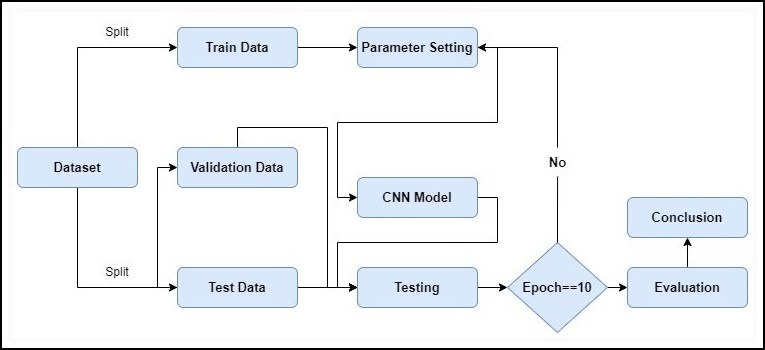
\includegraphics[width=8.8cm, height=4cm]{Tomato Final Flowchart.jpg}
\caption{Flowchart of the proposed work}
\label{fig: Figure 1}
\end{figure}

\subsection{Data Pre-Processing}
There isn't much extra effort required to normalise the photos because the PlantVillage collection already has pre-processed images with minimal to no distortion.\\
Additionally, to enhance the dataset size and improve the resilience of the CNN model, data augmentation methods including rotation, flipping, and zooming were used to the training set.\\
Overall, the data employed in this effort to classify potato leaf disorders is extensive, varied, and indicative of many different potato illnesses.




% \subsection{Temporal Attention module}
% Inspired by the various attention techniques~\cite{.....}, we employ a temporal attention module to capture temporal dependencies among snippets. After that, the attention scores are multiplied with the feature vectors to detect anomaly events. Thus, the temporal attention module allows the network to concentrate on the more important snippets.


\subsection{CNN - Convolutional Neural Network}

Convolutional neural networks (CNNs) are a type of sophisticated neural network that are mostly used for processing visual input like images and movies. They have shown to be highly helpful in tasks requiring image and video processing due to their several levels. The model's convolutional layers employ trainable filters to pull out crucial information from the input photographs. Pooling layers reduce the computational cost of these acquired properties. Fully connected layers are utilised to correctly classify the input by mapping the returned attributes to the appropriate output classes. CNNs have revolutionised computer vision through their application in object detection, semantic segmentation, and image classification. Recent research has focused on using CNNs to automatically recognise and classify plant diseases, notably those that affect tomato leaves. When compared to well-known deep learning architectures like AlexNet and GoogleNet, customised variations of the ResNet architecture have been demonstrated to be the most accurate.\\

The ResNet50 architecture, initially proposed by Zhang et al. in a 2015 study \cite{Zhang_2021_WACV}, served as the foundation for our deep neural network model.

The basic concept of ResNet is the introduction of residual connections, which allow information to flow freely across different levels and across the network. This is accomplished by generating skip connections, which encourage a more efficient information flow by linking one layer's input to another's output, so providing a shortcut.\\

ResNet successfully resolves the issue of vanishing gradients typically encountered in deep neural networks by exploiting skip connections. The effectiveness of deep network training is increased by these connections, which enable more uniform gradient flow during backpropagation. ResNet enables more efficient training of very deep networks and improved gradient propagation as a consequence.\\

ResNet is a well-liked and extensively utilised architecture that comes in a variety of forms. ResNet50 stands out among these forms with its amazing 50-layer structure. In a variety of visual computing tasks, including scene segmentation, object tracking, and picture identification, ResNet50 has displayed outstanding performance. Its extraordinary talents have raised standards and resulted in substantial breakthroughs in a variety of disciplines.

\section{Experiment}
\subsection{Dataset}
The study used the 54,000 tagged images from 14 different crop types in the publicly available PlantVillage dataset. There were a total of 2,475 images of bell pepper leaves, each measuring 256 by 256 pixels. From the photographs of bell pepper leaves, two classes were made, one showing healthy leaves and the other one depicting disease stages. For simpler analysis, the dataset was divided into three subsets: the training set, which included 70\% of the pictures; the test set, which included 15\% of the photographs; and the validation set, which also included 15\% of the photographs. Each image in the dataset was captured in the JPEG format and represented using the RGB colour space, as seen in Figure~\ref{fig: Figure 2}.


 \begin{figure}[H]
 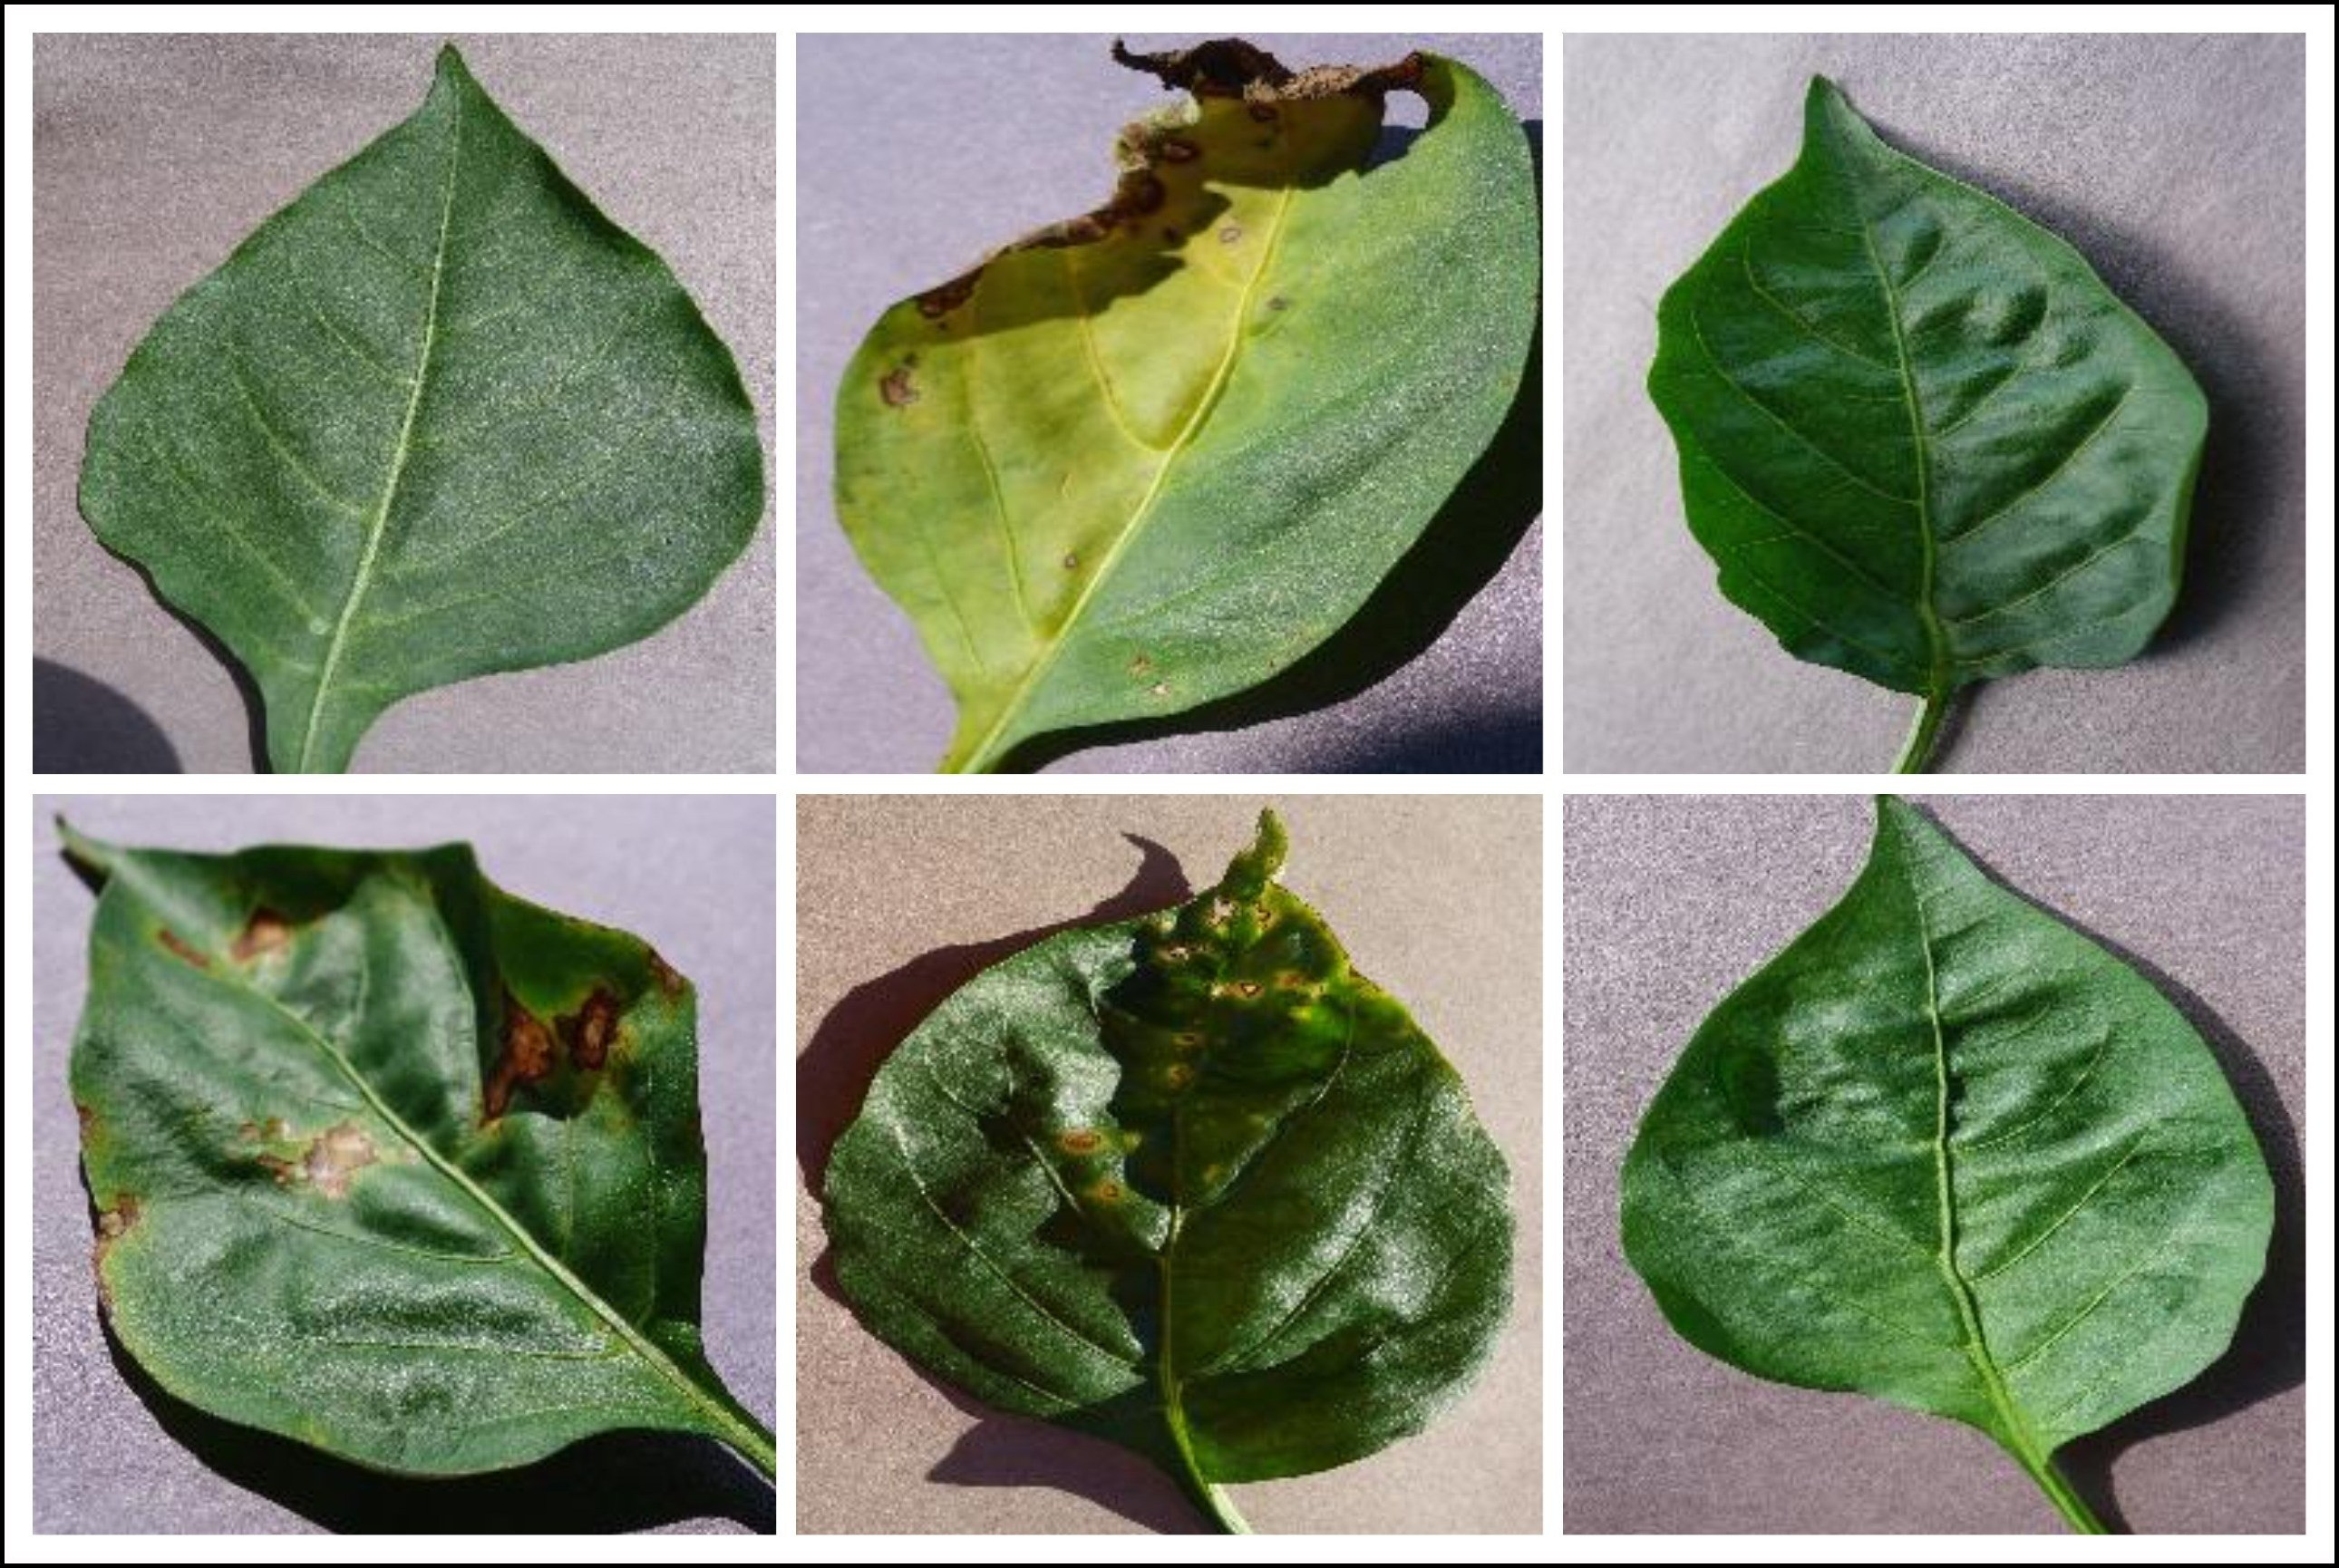
\includegraphics[width=8.8cm, height=5cm]{dataset.jpg}
\caption{Images from the datasets used}
\label{fig: Figure 2}
\end{figure}
 
\subsection{Evaluation Measure}
The performance of the recommended CNN model in identifying bell pepper leaf diseases was evaluated using a number of assessment measures, with classification accuracy serving as the primary indication. This statistic determines the percentage of the test set's images that were correctly identified when compared to all of the images.\\ 


Along with accuracy, a range of metrics like recall, precision, and F1-score are used to assess the suggested model's efficacy. Precision measures the association between accurately expected positive occurrences and all real positive instances, whereas recall measures the relationship between correctly predicted positive cases and all projected positive instances. The F1-score, a thorough statistic, is used to compute the harmonic mean of accuracy and recall.\
A combination of these assessment criteria may be used to assess the proposed CNN model's capability to distinguish between different bell pepper leaf diseases. They can also be used to compare the proposed CNN model to other models that are already in use.


\subsection{Experiment setting} 
The suggested CNN model is developed using Python and a variety of libraries, such as TensorFlow, Keras, and OpenCV, to identify leaf diseases in potato plants. The computer system utilised to operate the model is powered by an i7-6800 CPU operating at 3.4 GHz, a 2 GB NVIDIA GeForce GPU, and 16 GB of RAM. The model is trained with the Adaptive Moment Estimation optimizer across 10 epochs with a learning rate of 0.001 and a batch size of 32. The collection of bell pepper leaf images is divided into three sets: a training set, a validation set, and a testing set, each having relative proportions of 70\%, 15\%, and 15\%.


\section{Results and Discussion}
% In this section, we present and discuss the experimental results obtained 

The effectiveness of the model was evaluated using a number of metrics, including the F1-score, recall, accuracy, precision, and confusion matrix. The reported training accuracy was 97.8\%, however the highest validation accuracy recorded was 94.7\%. The model has a validation accuracy of 98\% percent and generally handled classification tasks effectively.

 \begin{figure}[H]
 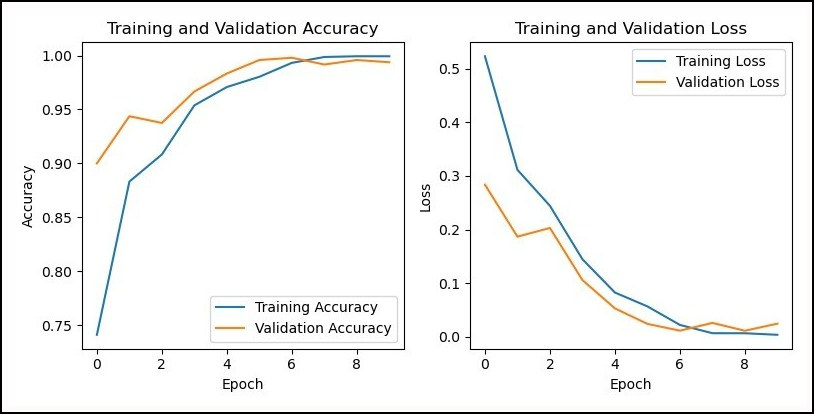
\includegraphics[width=8.9cm, height=4.5cm]{accuracy.jpg}
\caption{The model's accuracy  and loss was assessed during both the training and validation stages.}
\label{fig: Figure 3}
\end{figure}

The graphs visually show the accuracy and loss of the model. The loss graph exhibited a progressive decline in loss before doing the same, while the accuracy graph, as illustrated in Figure~\ref{fig: Figure 3}, revealed a steady increase in accuracy before stabilising. These graphs show the model's effectiveness and show that it may be a useful tool for classifying the 10 distinct varieties of tomato leaf diseases. By providing a crystal-clear picture of the model's evolution, these graphs enhance our understanding of the model's capabilities and reinforce its value as a reliable tool for sickness classification.


 \begin{figure}[H]
 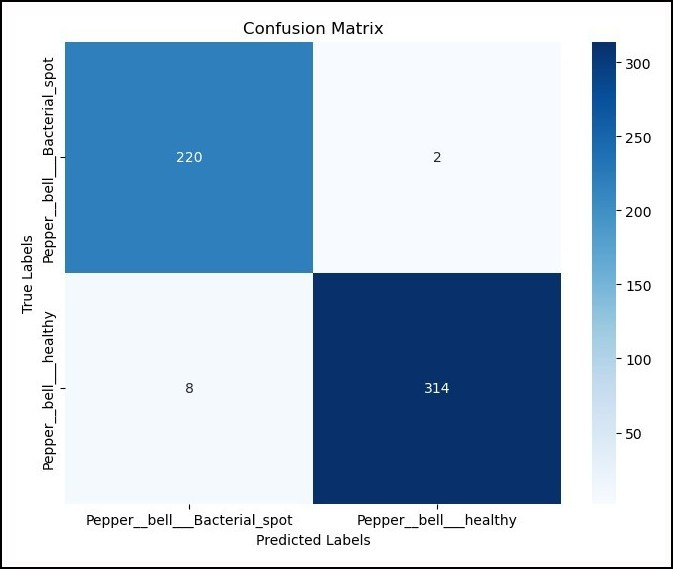
\includegraphics[width=8.8cm, height=5cm]{confusion.jpg}
\caption{Confusion matrix for the model used in the paper}
\label{fig: Figure 4}
\end{figure}

 \begin{figure}[H]
 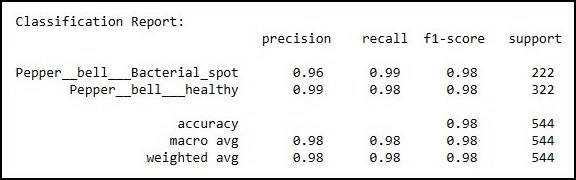
\includegraphics[width=8.8cm, height=4cm]{stats.jpg}
\caption{Accuracy, Precision, Recall and F1-Score for the used model}
\label{fig: Figure 5}
\end{figure}

We carefully evaluated image classification models using the confusion matrix and other performance measures, including accuracy, precision, recall, and F1 score. The confusion matrix provided a visual evaluation of the model's performance by comparing the predicted labels with the actual labels. The confusion matrix was used to calculate the accuracy, which measures the classification's overall correctness. The model's balance of recall and accuracy was also taken into account when calculating the F1 score; this is shown in figure~\ref{fig: Figure 4} and figure~\ref{fig: Figure 5}, respectively. Recall evaluated the model's ability to properly identify positive cases, whereas precision evaluated its capability to accurately identify all positive instances.

  
\section{Conclusion and Future Work}
Crop disease detection is crucial for the sustainable growth of the agricultural industry in India, which supports a significant portion of the population. Similar to tomatoes, potatoes are susceptible to various diseases that hinder their growth and productivity. In this study, a convolutional neural network (CNN) model is employed to propose a straightforward approach for identifying and diagnosing diseases affecting potato leaves, utilizing the Plant Village dataset. By analyzing leaf images and detecting patterns and characteristics, the model achieves impressive accuracy rates of 95-98\% while utilizing minimal computational resources. The model's robustness and performance are further enhanced through the implementation of data augmentation techniques. To further improve the model's performance, future research can explore alternative optimizers, learning rates, and novel architectures. Optimizing training parameters can also reduce training timeframes. This methodology extends beyond potatoes and can be adapted for disease detection in other plants such as apples, brinjal, and cucumbers.

% \section*{Acknowledgment}
% This work is supported by the FIST project of Department of Science and Technology, Govt. of India. We thank Mr. xxxxxxxxxxxxxxxxxx for his assistance with language editing, and proofreading. 
%\section{References}
\bibliographystyle{IEEEtran}
\bibliography{santos_bib}

\end{document}







